\documentclass{fkssolpub}

\usepackage[czech]{babel}
\usepackage{fontspec}
\usepackage{fkssugar}
\usepackage{amsmath}
\usepackage{graphicx}

\author{Ondřej Sedláček}
\school{Gymnázium Oty Pavla} 
\series{2p}
\problem{7} 

\begin{document} 

\begin{figure}[h!]
  \centering
  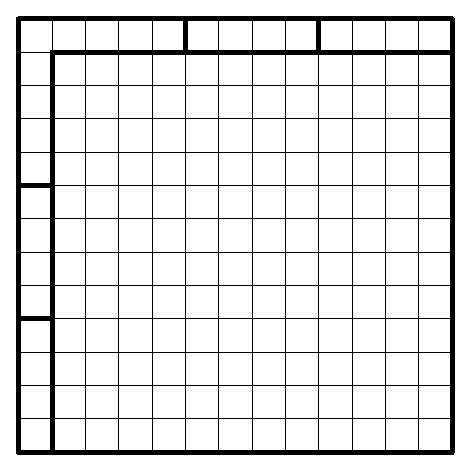
\includegraphics{7-fig}
  \caption{Nejlepší řešení s pěti řezy}
\end{figure}

Na obrázku výše můžeme vidět nejlepší řešení, které dosáhneme pomocí celkem
pěti řezů.

Protože jeden ze čtverců, který skládáme, má šířku o jednu menší než ten řezaný čtverec
($13 - 12 = 1$), když uřízneme z řezané tabulky obdélník o kratší straně delší než 1,
vznikne v řezané tabulce "díra", kterou budeme muset doplnit, abychom mohli sestrojit
čtverec o šířce 12. Proto tímto způsobem nemůžeme snížit počet řezů.

\end{document}
